\documentclass[10pt,handout]{beamer}
%\documentclass[10pt]{beamer}
\usetheme{Boadilla}
\usepackage[utf8]{inputenc}
\usepackage{amsmath}
\usepackage{amsfonts}
\usepackage{amssymb}
\usepackage{tikz}
\usetikzlibrary{arrows,decorations.markings}
\usetikzlibrary{shapes.geometric}
\usetikzlibrary{positioning}
\usepackage[absolute,verbose,overlay]{textpos}
\usepackage{stackengine}
\usepackage{scalerel}
\usepackage{tikz-uml}
\usepackage{listings}
\usepackage{forest}
\usepackage{booktabs}
\usepackage{listings}
\usepackage{fancyvrb}
\usepackage{pgfplots}
\usepackage{stmaryrd}

\usepackage{amsmath}
\usepackage{algorithm}
\usepackage[noend]{algpseudocode}
\usepackage{mathtools}

\lstset { %
    language=C++,
    backgroundcolor=\color{blue!10}, % set backgroundcolor
    basicstyle=\footnotesize,% basic font setting,
        commentstyle=\color[rgb]{0.026,0.112,0.095},
                basicstyle=\ttfamily,
                keywordstyle=\color{blue}\ttfamily,
                stringstyle=\color{red}\ttfamily,
                commentstyle=\color{gray}\ttfamily,
                morecomment=[l][\color{magenta}]{\#}
}

\graphicspath{{figures/}}


\newlength\triwidth
\author{\href{mailto:julian.erhard@tum.de}{Julian Erhard}, \href{mailto:j.gottfriedsen@tum.de}{Jakob Gottfriedsen}, \href{mailto:petermuench@mytum.de}{Peter Munch}, \href{mailto:a.roschlaub@tum.de}{Alexander Roschlaub}, \href{mailto:m.schwarz@tum.de}{Michael Schwarz}}
\title{Value Set Analysis in LLVM}
%\setbeamercovered{transparent} 
%\setbeamertemplate{navigation symbols}{} 
%\logo{} 
\institute{IN2053 - Program Optimization Lab 2018} 
%\date{February 8, 2017} 
%\subject{} 

\setbeamertemplate{footline}[frame number]{}

%gets rid of bottom navigation symbols
\setbeamertemplate{navigation symbols}{}
\expandafter\def\expandafter\insertshorttitle\expandafter{%
  \insertshorttitle\hfill%
  \insertframenumber\,/\,\inserttotalframenumber}

%gets rid of footer
%will override 'frame number' instruction above
%comment out to revert to previous/default definitions
%\setbeamertemplate{footline}{}

\setbeamertemplate{bibliography item}{}



\bibliographystyle{apalike}
% make bibliography entries smaller
%\renewcommand\bibfont{\scriptsize}
% If you have more than one page of references, you want to tell beamer
% to put the continuation section label from the second slide onwards
\setbeamertemplate{frametitle continuation}[from second]
% Now get rid of all the colours
\setbeamercolor*{bibliography entry title}{fg=black}
\setbeamercolor*{bibliography entry author}{fg=black}
\setbeamercolor*{bibliography entry location}{fg=black}
\setbeamercolor*{bibliography entry note}{fg=black}

\begin{document}

\begin{frame}
\titlepage
\end{frame}

%\begin{frame}
%\tableofcontents
%\end{frame}

\newcommand{\linen}[2]{ &&\qquad #1 & #2 \\}
\newcommand{\linenn}[4]{#1 & #2 &\qquad #3 & #4 \\}
\newcommand{\linel}[1]{ &&#1 \\}

\usetikzlibrary{decorations.text}
\definecolor{mygray}{RGB}{208,208,208}
\definecolor{mymagenta}{RGB}{226,0,116}
\newcommand*{\mytextstylee}{\sffamily\bfseries\color{white!85}}
\newcommand*{\mytextstyle}{\sffamily\bfseries\color{black!85}}
\newcommand{\arcarrow}[3]{%
   % inner radius, middle radius, outer radius, start angle,
   % end angle, tip protusion angle, options, text
   \pgfmathsetmacro{\rin}{2.5}
   \pgfmathsetmacro{\rmid}{3.0}
   \pgfmathsetmacro{\rout}{3.5}
   \pgfmathsetmacro{\astart}{#1}
   \pgfmathsetmacro{\aend}{#2}
   \pgfmathsetmacro{\atip}{5}
   \fill[mygray, very thick] (\astart+\atip:\rin)
                         arc (\astart+\atip:\aend:\rin)
      -- (\aend-\atip:\rmid)
      -- (\aend:\rout)   arc (\aend:\astart+\atip:\rout)
      -- (\astart:\rmid) -- cycle;
   \path[
      decoration = {
         text along path,
         text = {|\mytextstyle|#3},
         text align = {align = center},
         raise = -1.0ex
      },
      decorate
   ](\astart+\atip:\rmid) arc (\astart+\atip:\aend+\atip:\rmid);
}
\newcommand{\arcarroww}[3]{%
   % inner radius, middle radius, outer radius, start angle,
   % end angle, tip protusion angle, options, text
   \pgfmathsetmacro{\rin}{2.5}
   \pgfmathsetmacro{\rmid}{3.0}
   \pgfmathsetmacro{\rout}{3.5}
   \pgfmathsetmacro{\astart}{#1}
   \pgfmathsetmacro{\aend}{#2}
   \pgfmathsetmacro{\atip}{5}
   \fill[blue, very thick] (\astart+\atip:\rin)
                         arc (\astart+\atip:\aend:\rin)
      -- (\aend-\atip:\rmid)
      -- (\aend:\rout)   arc (\aend:\astart+\atip:\rout)
      -- (\astart:\rmid) -- cycle;
   \path[
      decoration = {
         text along path,
         text = {|\mytextstylee|#3},
         text align = {align = center},
         raise = -1.0ex
      },
      decorate
   ](\astart+\atip:\rmid) arc (\astart+\atip:\aend+\atip:\rmid);
}

\lstset { %
    language=C++,
    backgroundcolor=\color{blue!10}, % set backgroundcolor
    basicstyle=\footnotesize,% basic font setting,
        commentstyle=\color[rgb]{0.026,0.112,0.095},
                basicstyle=\ttfamily,
                keywordstyle=\color{blue}\ttfamily,
                stringstyle=\color{red}\ttfamily,
                commentstyle=\color{gray}\ttfamily,
                morecomment=[l][\color{magenta}]{\#}
}
%--------------------------------------------------------------------------------------------------
%--------------------------------------------------------------------------------------------------
\begin{frame}[fragile]{\textcolor{blue}{Value Set Analysis}}

\underline{\smash{Bounded Set Analysis:}}
%\begin{itemize}
%\item
\begin{align*}
Var \,\rightarrow\,\{a,\,b,\,c,\,...\}_n
\end{align*}
%\end{itemize}

\underline{\smash{Interval Analysis:}}
%\begin{itemize}
%\item
\begin{align*}
Var \,\rightarrow\, [a:b]_n
\end{align*}
%\end{itemize}

\underline{\smash{Strided Interval Analysis:}}
%\begin{itemize}
%\item
\begin{align*}
Var \,\rightarrow\,s[a:b]_n
\end{align*}
%\end{itemize}

\vspace{1.5cm}

SSA: sufficient to store the {\color{blue}abstract value for each variable once per basic block}:\footnote{The need to store it not just once only arises to preserve information at conditional branches.}
\begin{align*}
\mathcal{D}\,:\, BB \,\rightarrow\, Var \, \rightarrow\, Val
\end{align*}

\end{frame}
%--------------------------------------------------------------------------------------------------

\begin{frame}[fragile]{\textcolor{blue}{Passes in LLVM}}
LLVM's analysis and optimization framework {\color{blue} opt}:


\vspace{2cm}
\begin{center}
Figure: stages of clang and LLVM
\end{center}
\vspace{2cm}


using existing passes (from command line):
\begin{footnotesize}
\begin{lstlisting}[language=C++]
opt -load -mem2reg -o hello-opt.bc < hello.bc
\end{lstlisting}
\end{footnotesize}
running user passes:
\begin{footnotesize}
\begin{lstlisting}[language=C++]
opt -load llvm/lib/llvm-vsa.so -vsapass -o hello.bc < hello.bc
\end{lstlisting}
\end{footnotesize}

\end{frame}

\begin{frame}[fragile]{\textcolor{blue}{Motivation}}
%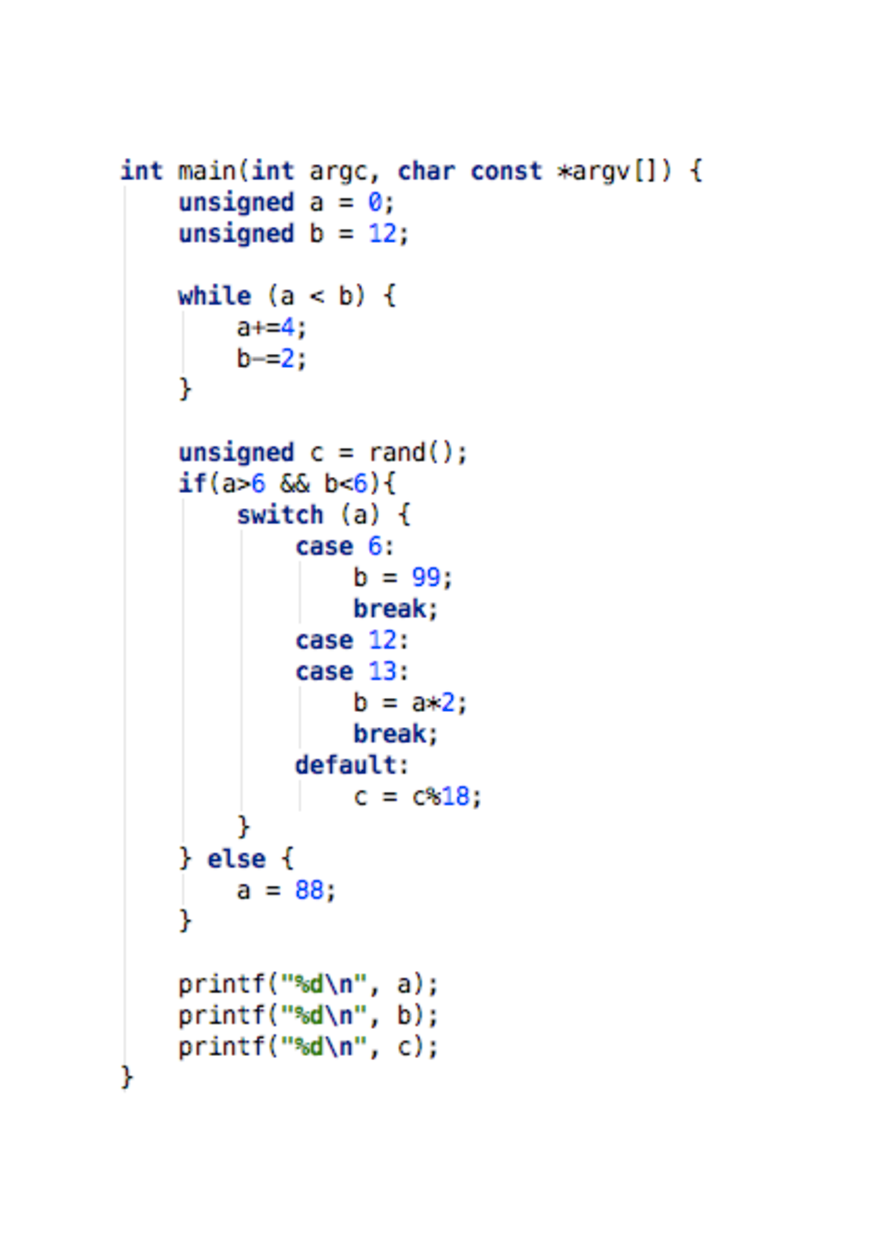
\includegraphics[scale=0.6]{src/example_c.pdf}
\begin{footnotesize}
\begin{lstlisting}[language=C++]
int main(int argc, char const *argv[]) {
    unsigned a = 0, b = 12, c = rand();

    while (a < b) { a+=4; b-=2; }

    if(a>6 && b<6){
        switch (a) {
            case  6: b = 99;  break;                 // reachable?
            case 12:
            case 13: b = a*2; break;
            default:
                c = c%18;
        }
    } else {
        a = 88;
    }

    printf("%d\n", a);		// what will/might be printed out?
    printf("%d\n", b);
    printf("%d\n", c);
}
\end{lstlisting}
\end{footnotesize}
\end{frame}

\begin{frame}[fragile]{\textcolor{blue}{LLVM's Intermediate Representation IR}}

\newcommand{\keyword}[1]{\textbf{\color{red} #1}}
\newcommand{\labele}[1]{\textbf{\underline{\smash{#1}}}}

\begin{scriptsize}
\begingroup
  \fontfamily{pcr}\selectfont
\keyword{define} dso\_local i32 @main(i31 \%argc, i8** \%argv) \#0 \{  \\
\labele{entry:} \\
\qquad \keyword{br} label \%while.cond \\

\vspace{0.2cm}

\labele{while.cond:} \\
\qquad   \%a.0 \keyword{= phi} i32 [ 0, \%entry ], [ \%add, \%while.body ] \\
\qquad   \%b.0 \keyword{= phi} i32 [ 12, \%entry ], [ \%sub, \%while.body ] \\
\qquad   \%cmp \keyword{= icmp} ult i32 \%a.0, \%b.0 \\
\qquad   \keyword{br} i1 \%cmp, label \%while.body, label \%while.end \\

\vspace{0.2cm}

\labele{while.body:} \\
\qquad     \%add \keyword{= add} i32 \%a.0, 4 \\
\qquad     \%sub \keyword{= sub} i32 \%b.0, 2 \\
\qquad     \keyword{br} label \%while.cond \\

\vspace{0.2cm}

\labele{while.end:} \\
\qquad     \%call = \keyword{call} i32 @rand() \#3 \\
\qquad     \%cmp1 = \keyword{icmp ugt} i32 \%a.0, 6 \\
\qquad     \keyword{br} i1 \%cmp1, label \%land.lhs.true, label \%if.else \\

\vspace{0.2cm}

\labele{land.lhs.true:} \\
\qquad     \%cmp2 \keyword{= icmp ult} i32 \%b.0, 6 \\
\qquad     \keyword{br} i1 \%cmp2, label \%if.then, label \%if.else


\endgroup

\end{scriptsize}

\vfill

\hfill ... and many more lines of code
\end{frame}

%--------------------------------------------------------------------------------------------------
\begin{frame}[fragile]{\textcolor{blue}{Passes in LLVM (cont.)}}
\underline{\smash{Creating user passes:}}
\begin{itemize}
\item inherit from existing passes (module, function, block):
\begin{footnotesize}
\begin{lstlisting}[language=C++]
struct ThisPass : public ModulePass {}
\end{lstlisting}
\end{footnotesize}

\item specify required passes, which have to be run in advance:
\begin{footnotesize}
\begin{lstlisting}[language=C++]
void ThisPass::getAnalysisUsage(AnalysisUsage &AU) override {
  AU.setPreservesAll();
  AU.addRequired<OtherPass>();
}
\end{lstlisting}
\end{footnotesize}

\item perform analysis by using/accessing results of other passes:
\begin{footnotesize}
\begin{lstlisting}[language=C++]
bool ThisPass::runOnModule(Module &M) override {
  auto& other_result =
    getAnalysis<OtherPass>(function).getResult();
  /* ... perform analysis and fill result ... */

  // Return if the pass modified the bitcode (no)
  return false;
}
\end{lstlisting}
\end{footnotesize}

\item make results available for other pass (optional):
\begin{footnotesize}
\begin{lstlisting}[language=C++]
ThisResult& ThisPass::getResult(){ return result; }
\end{lstlisting}
\end{footnotesize}

\end{itemize}

\end{frame}
%--------------------------------------------------------------------------------------------------
%\begin{frame}[fragile]{\textcolor{blue}{LLVM's Intermediate Representation IR}}
%\begin{center}
%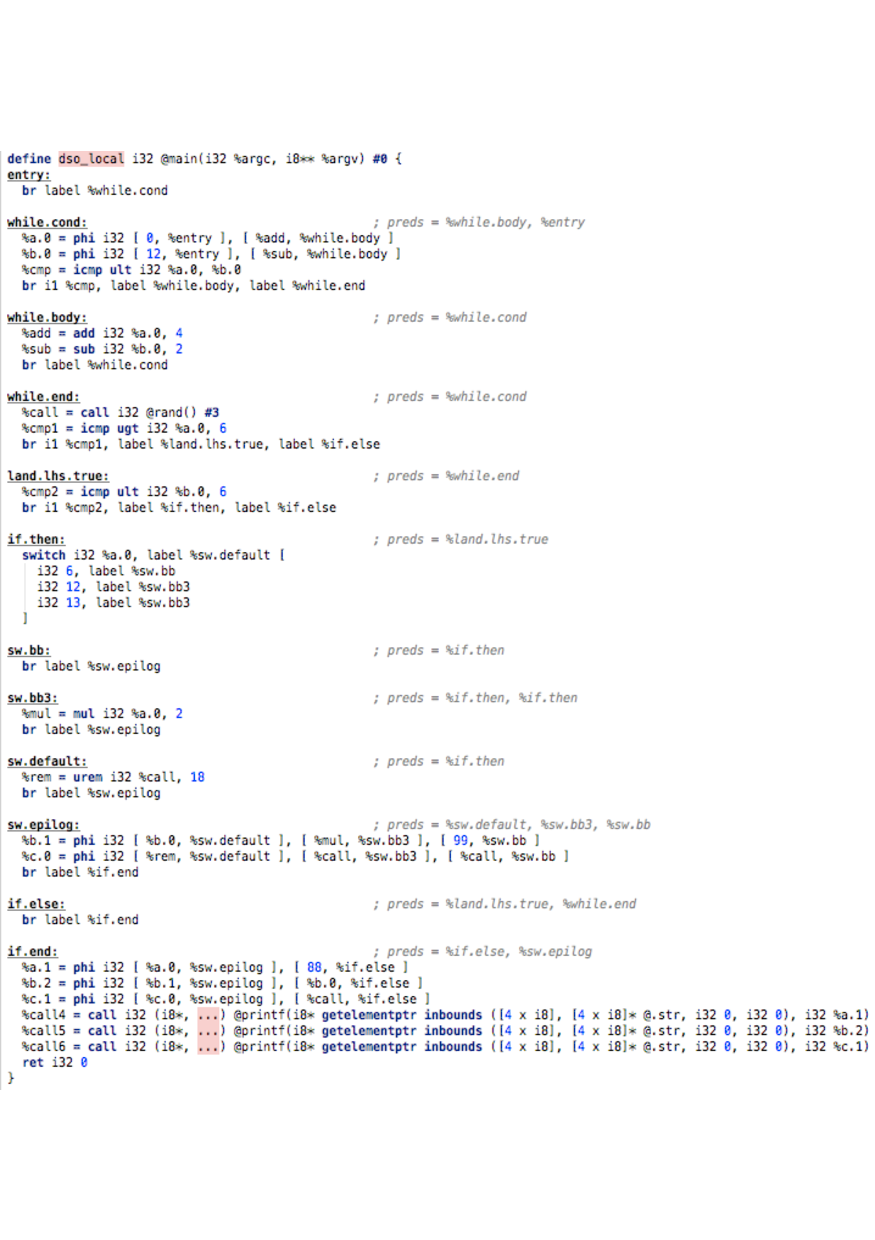
\includegraphics[width=0.7\textwidth, trim={0.1cm 12cm 4.5cm 2.5cm},clip]{src/example_ll.pdf}
%\end{center}
%
%\hfill ... and many more lines of code
%\end{frame}



%--------------------------------------------------------------------------------------------------
\begin{frame}[fragile]{\textcolor{blue}{Content of the Lab}}

\underline{Tasks:}
\begin{itemize}
\item implement {\color{blue}abstract domain}s that suitably represent value sets
\item develop a new analysis tool in LLVM to determine the value set of each \\
\qquad variable, using visitor and fixpoint algorithm (worklist) $\triangleright$ {\color{blue} VSAPass}
\item make results accessible via API: {\color{blue} VSAResult} and {\color{blue} VSAResultValue}
\item compare results with LLVM's {\color{blue} LazyValueInfo}
\end{itemize}

\vspace{1cm}

\underline{\smash{Future work:}}
\begin{itemize}
\item widening and narrowing
\item inter-procedural analysis
\item memory access
\end{itemize}
\hfill unknowns (ops, return values and arguments of functions) treated as: {\color{blue} $\top$}

\end{frame}
%--------------------------------------------------------------------------------------------------

\begin{frame}

Part 1:
\vspace{0.2cm}

{\LARGE \textbf{\textcolor{blue}{Abstract Domain}}}

\end{frame}




\begin{frame}[fragile]{\textcolor{blue}{Background to LLVM Integer Types}}
\begin{itemize}
\item In LLVM the type of $N$-bit integers is the set $\texttt{i}N \coloneqq \{0,1\}^N, \text{for~} N \in \{1,\dots, 2^{23}-1\}$.
\item "$\texttt{i}N \cong \mathbb{Z}/2^N$~" 
\item In the in-memory-representation, these types are represented by the LLVM class APInt.
\item This type is used for both signed and unsigned integers.
 
\item We use APInt 	 in our implementation of abstract domains.

\end{itemize}

\end{frame}

\begin{frame}[fragile]{\textcolor{blue}{LLVM Integer Operations}}
\begin{large}Arithmetic Operations:\end{large} \\
In LLVM there are separate $\texttt{div}$ and $\texttt{rem}$ operations for signed and unsigned integers. 
For $\texttt{add}$, $\texttt{sub}$ and $\texttt{mul}$, there is no such distinction needed.
\begin{itemize}
\item $\texttt{<result> = add [nuw] [nsw] <bitWidth> <op1> <op2>}$
\item $\texttt{<result> = sub [nuw] [nsw] <bitWidth> <op1> <op2>}$
\item $\texttt{<result> = mul [nuw] [nsw] <bitWidth> <op1> <op2>}$
\item $\texttt{<result> = udiv [exact] <bitWidth> <op1> <op2>}$ 
\footnote{\label{not-impl} $\texttt{exact}$-flag not used in our implementation.}
\item $\texttt{<result> = sdiv [exact] <bitWidth> <op1> <op2>} ^{~\ref{not-impl}}$
\item $\texttt{<result> = urem <bitWidth> <op1> <op2>}$
\item $\texttt{<result> = srem <bitWidth> <op1> <op2>}$
\end{itemize}

$\texttt{nuw}$ : "no unsigned wrap", $\texttt{nsw}$ : "no signed wrap"

\end{frame}

\begin{frame}[fragile]{\textcolor{blue}{LLVM Integer Operations, Continued}}
Bitwise Operations:
\begin{itemize}
\item $\texttt{<result> = shl [nuw] [nsw] <bitWidth> <op1> <op2>}$
\item $\texttt{<result> = lshr [exact] <bitWidth> <op1> <op2>}$ \footnote{\label{not-impl2} $\texttt{exact}$-flag not used in our implementation.}
\item $\texttt{<result> = ashr [exact] <bitWidth> <op1> <op2>}^{~\ref{not-impl2}}$
\item $\texttt{<result> = and <bitWidth> <op1> <op2>}$
\item $\texttt{<result> = or <bitWidth> <op1> <op2>}$
\item $\texttt{<result> = xor <bitWidth> <op1> <op2>}$
\end{itemize}

\end{frame}

\begin{frame}[fragile]{\textcolor{blue}{Bounded Set}}
\begin{itemize}
\item A bounded set represents a set of values up to a given cardinality $k$, or $\top$: \\
$\mathrm{BS}_{N} \coloneqq \{M\in \mathcal{P}(\texttt{i}N)\mid |M| \leq k\} \dot\cup \{ \top \}$ \\
\item $\sqcup$ and $\sqsubseteq$ on bounded sets essentially reduce to $\cup$ and $\subseteq$ on sets.
\item Any set with more elements than $k$ is over-approximated by $\top$.
\item $\gamma_{BS_N} \colon \mathrm{BS}_N \rightarrow \mathcal{P}(\texttt{i}N),
b \mapsto
\begin{cases}
\texttt{i}N,  & \text{if }b=\top \\
b, & \text{otherwise}
\end{cases}
$ 

\end{itemize}

\end{frame}


\begin{frame}[fragile]{\textcolor{blue}{Modular Strided Interval}}
\begin{itemize}

\item Intervals:
\begin{itemize}
\item $\mathrm{I} \coloneqq [a,b], \text{for } a,b \in \mathbb{Z}$
\end{itemize}
\item Strided Intervals:
\begin{itemize}
\item $\mathrm{SI} \coloneqq s[a,b], \text{for } a,b \in \mathbb{Z}, s \in \mathbb{N}$
\item $\gamma_{\mathrm{SI}}, s[a,b] \mapsto \{k \in \mathbb{Z} \mid
a \leq k \leq b, k \equiv a \mod s \}$
\end{itemize}
\item Modular Strided Intervals:
\begin{itemize}
\item $\mathrm{MSI}_{N} \coloneqq \{\overline{s}[\overline{a},\overline{b}]_N \mid \overline{a}, \overline{b}, \overline{s} \in \mathbb{Z}/2^N \} \dot\cup \{\bot\}$
\item $\gamma_{\mathrm{MSI}_N}, s[a,b]_N \mapsto \{k + 2^N\mathbb{Z} \mid
k \in \mathbb{Z}, a \leq k \leq z, k \equiv a \mod s \}$, \\ where $z = \min\{l \in \mathbb{Z} \mid l \geq a, l \equiv b \mod 2^N \}$
\item Examples:
\begin{itemize}
\item $12[15,63]_8 \stackrel{\gamma~}{\rightarrow}\{15,27,39,51,63\} \subseteq \mathbb{Z}/2^8$
\item $4[10,6]_4 \stackrel{\gamma~}{\rightarrow}\{10,14,2,6\} \subseteq \mathbb{Z}/2^4$

\end{itemize}
\end{itemize}
\end{itemize}

\end{frame}


\begin{frame}[fragile]{\textcolor{blue}{Modular Strided Interval: Normalization}}
Note that the representation of a set by a modular strided interval may not be unique. Thus, we introduce a predicate \textit{normal}, such that there is always a unique \textit{normalized} representation.
Example:
\begin{flalign*}
& \rlap{\(\mathrm{normal}_N(\overline{s}[\overline{a}, \overline{b}]_N) \leftrightarrow (\)} &
\end{flalign*}
\begin{flalign*}
\quad & \overline{s} = 0 \leftrightarrow \overline{a} = \overline{b} & \\
\quad \land\ & \overline{b} \in \gamma_N(\overline{s}[\overline{a}, \overline{b}]_N) & \\
\quad \land\; & \overline{a} = \min\{a' \in \{0 \ldots 2^N-1\} \ldotp \gamma_N(\overline{s}[\overline{a'}, \overline{b}]_N) = \gamma_N(\overline{s}[\overline{a}, \overline{b}]_N)\} + 2^N \mathbb{Z} &
\end{flalign*}
\begin{flalign*}
& ) &
\end{flalign*}
\end{frame}

\begin{frame}[fragile]{\textcolor{blue}{Modular Strided Interval: Union}}
Modular strided intervals do not form a lattice, as, in general, there is no least upper bound of two elements. \\
Example: 
\end{frame}
\begin{frame}[fragile]{\textcolor{blue}{Abstract Domain Class Structure}}

\begin{center}
\begin{tikzpicture}[thick,scale=0.8, every node/.style={transform shape}]

\umlinterface[]{AbstractDomain}{
}{ 
add(other) : AbstractDomain \\ /* other arithmetic and logical operations */ \\ \\

icmp(other, predicate) : (AbstractDomain, AbstractDomain) \\ \\
leastUpperBound(other) : AbstractDomain \\ 
lessOrEqual(other) : bool \\
}

\umlclass[x=-3.5,y=-4.0]{CompositeDomain}{delegate : AbstractDomain}{}
\umlclass[x=+2.5,y=-4.0]{BoundedSet}{
values : set$<$APInt$>$ \\
isTop : bool}{}
\umlclass[x=+3.0,y=-6.0]{StridedInterval}{
min, max, stride : APInt \\
isBottom : bool}{}


%\umlclass[x=-3,y=-6.5]{OperationNDim$<$vec$>$}{}{}

%\umlclass[x=3,y=-6.5]{OperationNDim$<$novec$>$}{}{}

\umlinherit[geometry=|-]{CompositeDomain}{AbstractDomain}
\umlinherit[anchor1=north,anchor2=-41]{BoundedSet}{AbstractDomain}
\umlinherit[geometry=-|-, arm1=0.5cm,anchors=east and east]{StridedInterval}{AbstractDomain}
%\umlaggreg[]{OperationNDim$<$T;U;V$>$}{OperationMass}
%\umlaggreg[]{OperationNDim$<$T;U;V$>$}{OperationConvection}
\umlaggreg[]{CompositeDomain}{BoundedSet}
\umlaggreg[geometry=-|-,anchors=east and west]{CompositeDomain}{StridedInterval}


\end{tikzpicture}
\end{center}

\end{frame}

\begin{frame}[fragile]{\textcolor{blue}{Application Interface}}

\begin{minipage}{0.5\textwidth}
\begin{center}
\begin{tikzpicture}[thick,scale=0.8, every node/.style={transform shape}]

\umlclass[fill=red!20
%,y=+3
,y=+5, x=-6.5
]{VSAResult}{
}{ 
is\_reachable(basic\_block) : bool \\
is\_resultat\_available(bb, value) : bool \\
get\_abstract\_value() : VSAResultValue \\
}

\umlclass[fill=red!20
%,y=+3
,y=1.5, x=-6.5
]{VSAResultValue}{
}{ 
test(predicate, constant) : tristate \\
min() : int \\
max() : int \\
size() : int \\
constant() : int \\
is\_constant() : bool \\
}

\end{tikzpicture}
\end{center}
\end{minipage}
\begin{minipage}{0.49\textwidth}
\begin{itemize}
\item after a successful pass:\\
\quad {\color{blue} auto\& res = vsap.get\_result();}
\item query information related to \\basic block (reachable or not) and/or variable (abstract value)\\
%\quad {\color{blue} auto\& res = vsap.get\_result();}
\end{itemize}
\end{minipage}

\end{frame}

\begin{frame}[fragile]{\textcolor{blue}{Connection of the Results to the Internal Abstract Domain}}

\begin{center}
\begin{tikzpicture}[thick,scale=0.8, every node/.style={transform shape}]

\umlinterface[rectangle split parts=1, x=1.0]{AbstractDomain}{
}{}

\umlclass[x=-3.5,y=-3.5, rectangle split parts=1]{CompositeDomain}{}{}
\umlclass[x=+1.0,y=-3.5, rectangle split parts=1]{BoundedSet}{}{}
\umlclass[x=+2.0,y=-5.5, rectangle split parts=1]{StridedInterval}{}{}

\umlclass[fill=red!20
%,y=+3
,y=0.5, x=-6.5
]{VSAResultValue}{
}{ 
test(predicate, constant) : bool \\
min() : int \\
max() : int \\
size() : int \\
constant() : int \\
is\_constant() : bool \\
}

%\umlclass[x=-3,y=-6.5]{OperationNDim$<$vec$>$}{}{}

%\umlclass[x=3,y=-6.5]{OperationNDim$<$novec$>$}{}{}

\umlinherit[geometry=|-]{CompositeDomain}{AbstractDomain}
\umlinherit[anchor1=north,anchor2=south]{BoundedSet}{AbstractDomain}
\umlinherit[geometry=-|-, arm1=0.5cm,anchors=east and east]{StridedInterval}{AbstractDomain}
%\umlaggreg[]{OperationNDim$<$T;U;V$>$}{OperationMass}
%\umlaggreg[]{OperationNDim$<$T;U;V$>$}{OperationConvection}
\umlaggreg[]{CompositeDomain}{BoundedSet}
\umlaggreg[geometry=-|-,anchors=east and west]{CompositeDomain}{StridedInterval}

\umlaggreg[geometry=|-|,anchor1=north,anchor2=north,arm1=0.5cm]{VSAResultValue}{AbstractDomain}

\end{tikzpicture}
\end{center}

\end{frame}


\begin{frame}

Part 2:
\vspace{0.2cm}

{\LARGE \textbf{\textcolor{blue}{Fixpoint Algorithm \& Visitor}}}

\end{frame}


\begin{frame}[fragile]{\textcolor{blue}{Data Structures}}

\underline{\smash{Data structures maintained during the analysis}}:
\begin{itemize}
\item {\color{blue}state} of each basic block (goal):\hfill {\color{red}red: abstract domain}
\begin{align*}
\mathcal{D}\,:\, BB\rightarrow \underbrace{ \left( Var \rightarrow {\color{red}Val} \right)_{\perp} }_{state\,\mathcal{D}_{BB}}
\end{align*}
\item {\color{blue}branch conditions}:
\begin{align*}
\mathcal{C}\,:\, \underbrace{\left(BB\rightarrow XX\right)}_{edge} \rightarrow \underbrace{ \left( Var \rightarrow {\color{red}Val} \right)_{\perp} }_{\mathcal{C}_{BB\rightarrow XX}}
\end{align*}
\end{itemize}
\qquad$\rightarrow$ effect of a guard: \begin{align*}
\mathcal{D}_{XX} \gets \llbracket BB\,\rightarrow\,XX \rrbracket \, \mathcal{D}_{BB} = \mathcal{D}_{BB} \,\oplus\, \mathcal{C}_{BB\rightarrow XX}
\end{align*}
\end{frame}

\begin{frame}[fragile]{\textcolor{blue}{Fixpoint Algorithm: Worklist}}

We maintain a {\color{blue}worklist $\mathcal{W}$} of basic blocks to be (re)evaluated.

\begin{algorithm}[H]
\caption{Fixpoint algorithm}
\begin{algorithmic}[1]
\Procedure{Fixpoint}{Function}
\State $\mathcal{W}$.push(Function.front())\Comment{push entry basic block of function}
\State \textbf{while} $!\, \mathcal{W}.empty()$ \textbf{then}:
\State \qquad visit $\mathcal{W}$.pop()
\EndProcedure
\end{algorithmic}
\end{algorithm}

Fixpoint algorithm terminates iff $\mathcal{W}$ is empty: a fixpoint has been found.

\vfill

Following {\color{blue}initial and entry states} are used (forward analysis):
\begin{align*}
\mathcal{D}_0\,:\, BB\rightarrow \, \perp \quad \text{and}\quad
\mathcal{D}_{entry}\,:\, BB\rightarrow \, \left( Arg_i\rightarrow \top \right)
\end{align*}

\end{frame}



\begin{frame}[fragile]{\textcolor{blue}{Visitor: (Entering) Basic Block}}

Visiting a basic block is a two-step process:
\begin{enumerate}
\item setting up the (temporary) input state $\mathcal{N}_{BB}$ during entering 
\item visiting all its instructions
\end{enumerate}

\begin{algorithm}[H]
\caption{Enter basic block BB}  %MS: Missing:pruning?
\begin{algorithmic}[1]
\Procedure{Visit}{BB}%\Comment{T: syntax tree}
\State $\mathcal{N}_{BB}= \bigsqcup \left\lbrace \mathcal{D}_{XX} \oplus \mathcal{C}_{XX\rightarrow BB} \,|\, XX \in \text{prev}(BB)\,\wedge\,\mathcal{D}_{XX}\neq\, \perp \right\rbrace$
\State \textbf{for each} $instruction \in \text{instructions}(BB)$:
\State \qquad visit $instruction$
\EndProcedure
\end{algorithmic}
\end{algorithm}
%\vfill
%\underline{Implementation details:}
%\begin{itemize}
%\item Construct $\mathcal{N}_{BB}$ iteratively: $\mathcal{N}_{BB}^{i+1} \gets \mathcal{N}_{BB}^{i} \,\sqcup\, \{ ... \}$ with $\mathcal{N}_{BB}^{0}\gets\perp$
%\item if $\{...\}=\perp$: skip it
%\item three cases: 
%$\perp \sqcup\, x = x$,
%$x \,\sqcup \perp = x$, and
%$x \,\sqcup\, y$
%\end{itemize}
\underline{\smash{Explicitly considered instructions}}:
\begin{itemize}
\item terminators: (un)conditional jumps, switches
\item PHI nodes
\item binary expressions
\end{itemize}
\end{frame}


\begin{frame}[fragile]{\textcolor{blue}{Visitor: Leaving Basic Block at Terminator}}

{\color{blue}check for change} of the local state and save it in $\mathcal{D}$:
\begin{algorithm}[H]
\caption{Visit terminator}
\begin{algorithmic}[1]
\Procedure{Visit}{Terminator}%\Comment{T: syntax tree}
%\State $\mathcal{N}_{BB} \gets \mathcal{D}_{BB} \,{\color{red}\sqcup}\, \mathcal{N}_{BB}$
\State \textbf{if} $\mathcal{N}_{BB} \,{\color{red}\sqsubseteq}\, \mathcal{D}_{BB}$ \textbf{then}:\Comment {\color{red}red: delegated to abstract domain\color{black}}
\State \qquad \textbf{return}
\Comment state has not changed
\State $\mathcal{D}_{BB} \gets \mathcal{N}_{BB}$
\State \textbf{for each} $XX \in \text{next}(BB)$:
\State \qquad\textbf{if} reachable($BB,\,XX$) \textbf{then}:
%\Comment always true if not-cond. branch
\State \qquad\qquad $\mathcal{W}$.push($XX$)
\EndProcedure
\end{algorithmic}
\end{algorithm}
in the case of change ($\mathcal{N}_{BB} \not\sqsubseteq \mathcal{D}_{BB}$), {\color{blue}push all reachable successors}:
\begin{itemize}
\item unconditional branch: push all successors
\item {\color{blue}conditional branch/switch}: check if $\exists (\#\,\rightarrow\,\perp)\in \mathcal{C}_{BB \,\rightarrow\, XX}$
\end{itemize}
\end{frame}


\begin{frame}[fragile]{\textcolor{blue}{Visitor: Conditional Branch}}


\begin{algorithm}[H]
\caption{Visit conditional branch (terminator)}
\begin{algorithmic}[1]
\Procedure{Visit}{$\textsc{jmp}\,(x \,\square\,y\,?\, XX \,:\, YY$)}%\Comment{T: syntax tree}
%\State $\mathcal{C}_{BB} \gets \emptyset$
\State \textbf{if } isVar($x$) \textbf{then}:
\State \qquad$\mathcal{C}_{BB\rightarrow XX} \gets  \mathcal{C}_{BB\rightarrow XX} \oplus \left\lbrace  x\,\rightarrow\, \mathcal{N}_{BB}[x]\,\,\,{\color{red}\square^\#}\,\mathcal{N}_{BB}[y]
\right\rbrace$
\State \qquad$\mathcal{C}_{BB\rightarrow YY} \gets  \mathcal{C}_{BB\rightarrow YY} \oplus \left\lbrace  x\,\rightarrow\, \mathcal{N}_{BB}[x]\,{\color{red}!\square^\#}\,\mathcal{N}_{BB}[y]
\right\rbrace$
\State \textbf{if } isVar($y$) \textbf{then}:
\State \qquad ...
%\Comment update conditions
\State \textsc{VisitTerminator}()
\EndProcedure
\end{algorithmic}
\end{algorithm}
considered comparisons:
\begin{align*}
\square \in \{ =,\, \neq,\, < ,\,\le,\,\ge,\, > \}
\end{align*}




%\begin{algorithm}[H]
%\caption{Reachability of basic block $BBN$ from $BB$}
%\begin{algorithmic}[1]
%\Procedure{Reachable}{BB, BBN}%\Comment{T: syntax tree}
%\State \textbf{return} $\exists (\#\,\rightarrow\,\perp)\in \mathcal{C}_{BB}[BBN]$
%\EndProcedure
%\end{algorithmic}
%\end{algorithm}
\end{frame}



\begin{frame}[fragile]{\textcolor{blue}{Visitor: Switch}}

\begin{algorithm}[H]
\caption{Visit switch (terminator)}
\small
\begin{algorithmic}[1]
\Procedure{Visit}{$\textsc{switch}\,[x=a\,:\,XX][x=b\,:\,YY][x=c\,:\,YY][default\,:\,ZZ]$}%\Comment{T: syntax tree}
%\State $\mathcal{C}_{BB} \gets \emptyset$
\State $\mathcal{C}_{BB\rightarrow XX} \gets \left\lbrace  x\,\rightarrow\, \mathcal{N}_{BB}[x]\,{\color{red}=^\#}\,a
\right\rbrace$
\State $\mathcal{C}_{BB\rightarrow YY} \gets \left\lbrace  x\,\rightarrow\, (\mathcal{N}_{BB}[x]\,{\color{red}=^\#}\,b) \sqcup (\mathcal{N}_{BB}[x]\,{\color{red}=^\#}\,c)
\right\rbrace$
\State $\mathcal{C}_{BB\rightarrow ZZ} \,\gets \left\lbrace  x\,\rightarrow\, \mathcal{N}_{BB}[x]\,{\color{red}\backslash}\,\{a,\,b,\,c\}
\right\rbrace$
\State \textsc{VisitTerminator}()
\EndProcedure
\end{algorithmic}
\end{algorithm}


\end{frame}


\begin{frame}[fragile]{\textcolor{blue}{Visitor: Parallel Assignments at PHI Node}}

\begin{algorithm}[H]
\caption{PHI node in basic block BB}
\begin{algorithmic}[1]
\Procedure{Phi}{$x\gets [YY\,:y]\,[ZZ\,:z]$}%\Comment{T: syntax tree}
\State $\mathcal{N}_{BB}\gets\mathcal{N}_{BB}\oplus\left\lbrace x\,\rightarrow\, \left(\mathcal{D}_{YY} \,\oplus\,C_{YY\rightarrow BB} \right) [y] \,\sqcup\, \left(\mathcal{D}_{ZZ} \,\oplus\,C_{ZZ\rightarrow BB} \right)[z] \right\rbrace$
\EndProcedure
\end{algorithmic}
\end{algorithm}

\end{frame}


\begin{frame}[fragile]{\textcolor{blue}{Visitor: Binary Expressions}}

\begin{algorithm}[H]
\caption{Addition in basic block BB}
\begin{algorithmic}[1]
\Procedure{Binary}{$x\gets y \,\square\, z$}%\Comment{T: syntax tree}
\State $\mathcal{N}_{BB}\gets\mathcal{N}_{BB}\oplus\left\lbrace x\,\rightarrow\, \mathcal{N}_{BB}[y]\,{\color{red}\square^\#}\, \mathcal{N}_{BB}[z] \right\rbrace$
\EndProcedure
\end{algorithmic}
\end{algorithm}
considered binary instructions:
\begin{align*}
\square \in \{ +,\,-,\,\times,\, /,\, \%,\, \ll,\, \gg \}
\end{align*}

\end{frame}


\begin{frame}[fragile]{\textcolor{blue}{Visitor: Memory access and Not-implemented Operations}}

Data in memory is considered unknown.
\begin{algorithm}[H]
\caption{Load in basic block BB}
\begin{algorithmic}[1]
\Procedure{Visit}{$x\gets \textsc{load}(...)$}%\Comment{T: syntax tree}
\State $\mathcal{N}_{BB}\gets\mathcal{N}_{BB}\oplus\left\lbrace x\,\rightarrow\, \top \right\rbrace$
\EndProcedure
\end{algorithmic}
\end{algorithm}

\vspace{0.5cm}

\hfill Not-implemented operations of form $x\gets \#$ are treated {\color{blue}implicitly} in the same way.

\end{frame}

\begin{frame}

Part 3:
\vspace{0.2cm}

{\LARGE \textbf{\textcolor{blue}{Livedemo}}}

\end{frame}
\begin{frame}
\titlepage
\end{frame}


\end{document}